\documentclass[a4paper,11pt]{article}
\usepackage[utf8]{inputenc}
\usepackage[english]{babel} % Adds processing for some simple special characters.

% Packages for better page formatting and nice footnotes. %
\usepackage{fancyhdr} % Headers.
\usepackage{multicol} % Columns.
\usepackage[margin=0.75in]{geometry} % Margins.
\pagestyle{fancy}
\fancyhf{} % What does this do?
\lhead{Alexander S. Wheaton}
\rhead{\today}
\cfoot{\thepage}

% Title and author for title page. %

\title{AGN Host Properties}
\author{
    Alexander S. Wheaton\\
    School of Physics and Astronomy\\
    The University of Edinburgh\\
    s1572046@ed.ac.uk\break
}

% Utilities for fine-grained control over image insertion. %

\usepackage{graphicx} % Insert images.
\usepackage{float} % Images float in document environment.
\usepackage{wrapfig} % Image/tables in multicols with \wrapfigure or \wraptable.
\usepackage{caption} % Captions for single images.
\usepackage{subcaption} % Captions for simultaneous images.
\graphicspath{ {./img/} }

% Not sure what this is for. %

\usepackage{fullpage,epsf}
\usepackage{lipsum}

% Some utilities for scientific and mathematical writing. %

\usepackage{amsmath} % Nice matrices.
\usepackage{xfrac}   % Slant fractions and other utilities.
\usepackage{isotope} % Nice markup syntax for chemical symbols.
\usepackage{siunitx} % Formatting for numbers with SI units.
\DeclareSIUnit\parsec{pc}
\DeclareSIUnit\lightyear{ly}
% Utilities for manual kerning adjustment. %

\newcommand\K{\kern.05em} % Small amount of kerning.
\newcommand\KK{\kern.1em} % Medium amount of kerning.
\newcommand\KKK{\kern.2em} % Large amount of kerning.
\newcommand\KKKK{\kern.3em} % Very large amount of kerning.

% Bibliography and referencing style. Use style=draft for troubleshooting.
\usepackage[backend=bibtex,style=phys,sorting=nyt]{biblatex}
\addbibresource{references.bib}

% Page formatting.

\begin{document}

\thispagestyle{empty}                   % No numbers of title page
\epsfxsize=40mm                         % Size of crest
\begin{minipage}[b]{110mm}
    {\Huge\bf School of Physics\\ and Astronomy
    \vspace*{17mm}}
\end{minipage}
\hfill
\begin{minipage}[t]{40mm}
    \makebox[40mm]{
    
\includegraphics[width=40mm]{crest.eps}}
\end{minipage}
\par\noindent                                           % Centre Title, and name
\vspace*{2cm}
\begin{center}
    \Large\bf \Large\bf MPhys Project\\
    \Large\bf Astrophysics\\[10pt]                     % Change to MP/CP/Astro
    \LARGE\bf Bayesian Inference of Star Formation History in the Host Galaxies of Tidal Disruption Events
\end{center}
\vspace*{0.5cm}
\begin{center}
    \bf Alexander S. Wheaton\\
    \today
\end{center}
\vspace*{5mm}

\begin{abstract}
    \noindent In this paper I review some of the basic properties of active galactic nuclei (AGN) with emphasis on their tendency to be observed in host galaxies which are ``post-starburst.'' I discuss the physics of a second nuclear phenomenon, tidal disruption events (TDEs), in quiescent galaxies. I then present the spectra of eight such galaxies at $z < 0.1$ known to have recently hosted a tidal disruption event, observed with the XSHOOTER instrument on the Very Large Telescope (VLT). I use the \textsc{Bagpipes} Python module to explore the effects of different star formation history (SFH) parameterisations on observed host spectra. By ``blind-fitting'' simulated spectra with a known SFH, I identify assumptions about the form of SFH which must be made in order to reliably detect past starbust activity in a now quiescent galaxy. I apply these assumptions to the spectra of the aforementioned TDEs, and find that their SFHs share the statistical behaviour of AGN---that they tend to occur in host galaxies which are post-starburst.
\end{abstract}

\vspace*{1cm}

\subsubsection*{Declaration}
\begin{quotation}
  \noindent I declare that this project and report is my own work.
\end{quotation}

\hspace*{1cm}
Signature:\hspace*{1cm}\includegraphics[width=6cm]{signature_repaired.eps}
\hspace*{1cm}
Date: \today

\vfill
\noindent{\bf Supervisor:} Professor A. Lawrence, FRSE, FRaS
\hfill
22 Weeks

\newpage
\thispagestyle{empty}
\section*{Personal Statement}\label{sec:personal_statement}
\lipsum[1]

\newpage
\thispagestyle{empty}
\tableofcontents

\newpage
\setcounter{page}{1} % Set page number to 1
\section{Introduction}\label{sec:introduction}

Little summary here

\section{Theory \& Motivation}\label{sec:theory_and_motivation}
\subsection{Active Galactic Nuclei}\label{sec:active_galactic_nuclei}
The luminosity of most galaxies is dominated by stellar, gas, and dust emission. The stellar component is the aggregate of many stars at different temperatures emitting thermally as near-perfect blackbodies.\cite{Peterson_1997} The medium of interstellar gas emits thermally when heated by the host galaxy's constituent stars, and creates both absorption and emission features at the particular energies of common interstellar gases and metals. Larger grains of interstellar dust absorb and re-emit stellar light in the infrared region of the spectrum.\cite{Dyson_1997}

Differences between the spectra of elliptical and disk galaxies hinge mostly upon the age of their constituent stars. Ellipticals or ``early-types'' are characterised by red photometric colours associated with an older stellar population. The emit very little light at wavelengths less than \SI{4000}{\angstrom} and because their interstellar mediums are mostly comprised of hot ionised gas, their spectra feature mostly absorption lines typical of G- and K-type stars, with no emission lines.\cite{Mo_2010}

Disk or ``late-type'' galaxies are characterised by younger, bluer stars, neutral \isotope{HI} and molecular \isotope{H_2} hydrogen regions.Their spiral arms are defined by \isotope{HII} regions and dust features. The emit considerably more light at wavelengths below the \SI{4000}{\angstrom} break, in the blue and near-UV. Interstellar gas ionised by hot, young stars in these galaxies produces strong emission lines, such as the Balmer-series ($\mathrm{H\alpha}$, $\mathrm{H\beta}$, $\mathrm{H\gamma}$, and $\mathrm{H\delta}$), \isotope{OII} and \isotope{OIII} lines.\cite{Mo_2010}

A fraction ($\approx \sfrac{1}{3}$) of galaxies, however, feature tightly confined (\SI{10}{\kilo\parsec}) ``weak'' nuclear luminosity which is \textit{not} consistent with this model.\cite{McClure_2019} A smaller fraction ($\approx \sfrac{1}{100}$) exhibit nuclear luminosity which is a significant fraction of the host's stellar luminosity ($\approx 10\%$).\cite{Sparke_2000} These galaxies are said to have nuclei which are ``active'' and are referred to as active galactic nuclei (AGNs).\cite{McClure_2019}\cite{Peterson_1997}

Some AGN are sufficiently have power outputs many times that of a typical host galaxy. In these objects, luminosity from the nucleus completely obscures the host galaxy. These are believed to be exceptionally rare, and as such are only detected at very high redshifts. At such distances, they appear point-like or  ``quasi-stellar,'' and are so dubbed quasars.\cite{Peterson_1997}

Lower luminosity AGN fall into the broad categories of ``Seyferts'' and radio galaxies.\footnote{Additionally, a common and very low luminosity class of galaxies featuring low-ionisation nuclear emission regions (LINERs), the highly variable luminosity classes of BL Lac objects (blazars) and optically violent variables (OVVs), and narrow-line X-ray galaxies, which are Seyferts which are heavily reddened and extinguished by dust within the host.} Type 1 and 2 Seyferts typically occur in spiral galaxies, featuring broad and narrow emission lines, respectively. Broad-line radio galaxies (BLRGs) and narrow-line radio galaxies (NLRGs) are the elliptical analogues to Seyferts, but are additionally radio-loud.\cite{Peterson_1997}

In general, AGN exhibit several key characteristics:

\begin{itemize}
    \item highly luminous and compact appearance
    \item continuum luminosity which is not explicable by thermal emission
    \item variable luminosity over short timescales of days to months
\end{itemize}

Unlike the peaked blackbody emission from stars, AGN radiate across the entire electromagnetic spectrum, with a peak in the UV and secondary peaks in the near infrared and X-ray. The generally accepted explanation for continuum spectral emission of this magnitude is a hot accretion disk surrounding a supermassive black hole.\cite{Peterson_1997} As matter falls into the black hole, its potential energy is converted to kinetic, which is dissipated by viscosity in the accretion disk to thermal energy, which is then radiated. In this model, material in the disc at a range of different temperatures accounts for continuum emission, while Doppler shifting of light emitted by disc material travelling at a range of velocities creates broad emission lines.\cite{McClure_2019}

\textbf{TODO: Get numbers for luminosities in this section!}

\subsection{The Starburst-AGN Connection}\label{sec:starburst_agn_connection}

A significant fraction (HOW MANY?) of AGN exhibit signatures of recent, large-scale star formation. These signatures include exceptionally blue photometric colours and strong \isotope{HII}-region-type emission lines, presumably gas ionised by hot, young O- and B-type stars. They also feature strong radio emissions, consistent with a high number of recent supernovae remnants.\cite{Peterson_1997}

Seyfert/radio galaxy frequency comparison

andy review
star formation - black hole mass relation\cite{Veilleux_2008}
\cite{Mo_2010}
Galaxy evolution compared to stellar Evolution
\subsection{Tidal Disruption Events}\label{sec:tidal_disruption_events}
\subsection{The XSHOOTER Data}\label{sec:xshooter_data}

\begin{figure}[H]
  \centering
  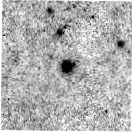
\includegraphics[width=0.3\textwidth]{ASASSN-14li_host_red}
  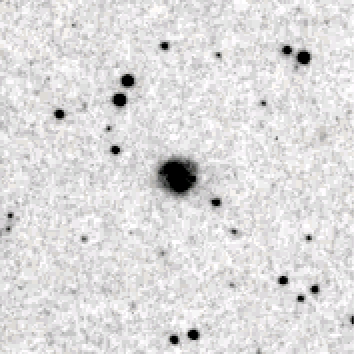
\includegraphics[width=0.3\textwidth]{AT2019qiz_host_red}
  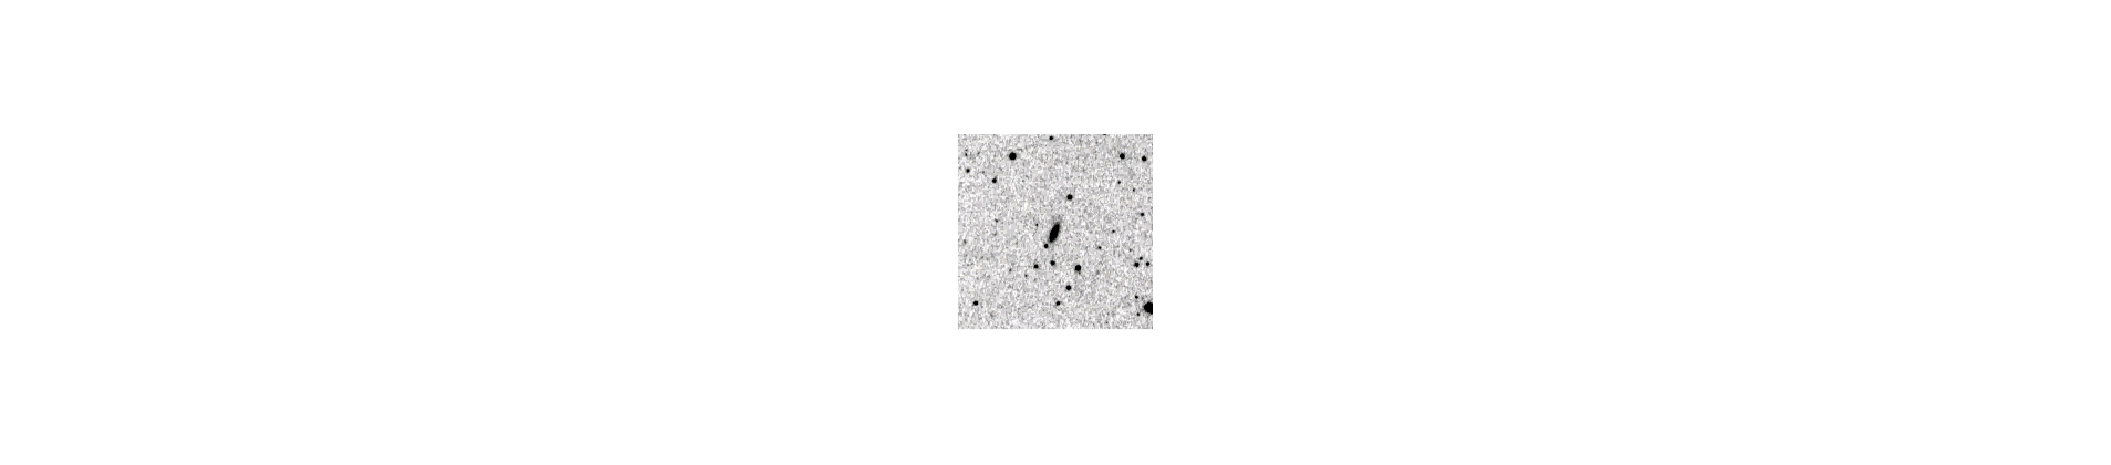
\includegraphics[width=0.3\textwidth]{iPTF16fnl_host_red}
  \caption{ASASSN-14li, AT2019qiz, and iPTF16fnl host galaxies.}
  \label{fig:xshooter_hosts}
\end{figure}

% Spare table with RAs and Decs included, although this is more information than needed.
% \begin{table}[H]
%   \begin{tabular}{l l c c c c r}
%     TDE         & Host Galaxy               & $\alpha$     & $\delta$     & $m$ & Morphology & $z$      \\
%     \hline \hline
%     ASASSN-14li & PGC 043234                & 12:48:15.23  & +17:46:26.44 & 15  & Compact    & 0.0206   \\
%     ASASSN-15oi & 2MASX J20390918-3045201   & 20:39:09.18  & -30:45:20.10 & 16  & Unresolved & 0.0484   \\
%     AT2018fyk   & LCRS B224721.6-450748     & 22:50:16.090 & -44:51:53.50 & 17  & Unresolved & 0.06     \\
%     AT2019ahk   & 2MASX J07001137-6602251   & 07:00:11.546 & -66:02:24.14 & 17  & E+A        & 0.026211 \\
%     AT2019azh   & KUG 0810+227              & 08:13:16.945 & +22:38:54.03 & 15  & E+A        & 0.022    \\
%     AT2019dsg   & 2MASX J20570298+1412165   & 20:57:02.974 & +14:12:15.86 & 15  & Unresolved & 0.0512   \\
%     AT2019qiz   & 2MASX J04463790-1013349   & 04:46:37.880 & -10:13:34.90 & 15  & Unresolved & 0.01513  \\
%     iPTF16fnl   & Markarian 950             & 00:29:57.010 & +32:53:37.24 & 16  & E+A        & 0.018    \\
%     \hline
%   \end{tabular}
%   \caption{XSHOOTER targets and their host morphologies on the Very Large Telescope (VLT).\cite{Zwicky_1975, Jose_2014, Holoien_2016a, Arcavi_2015, Holoien_2016b, Wevers_2021, Cacella_2019, Holoien_2019, van_Velzen_2019, Perez_Torres_2019, Seibert_2019, Gezari_2016, Blagorodnova_2017}}
%   \label{tab:xshooter_data}
% \end{table}

\begin{table}[H]
  \centering
  \begin{tabular}{l l c c r}
    TDE         & Host Galaxy             & $m$ & Morphology & $z$      \\
    \hline \hline
    ASASSN-14li & PGC 043234              & 15  & Compact    & 0.0206   \\
    ASASSN-15oi & 2MASX J20390918-3045201 & 16  & Unresolved & 0.0484   \\
    AT2018fyk   & LCRS B224721.6-450748   & 17  & Unresolved & 0.06     \\
    AT2019ahk   & 2MASX J07001137-6602251 & 17  & E+A        & 0.026211 \\
    AT2019azh   & KUG 0810+227            & 15  & E+A        & 0.022    \\
    AT2019dsg   & 2MASX J20570298+1412165 & 15  & Unresolved & 0.0512   \\
    AT2019qiz   & 2MASX J04463790-1013349 & 15  & Unresolved & 0.01513  \\
    iPTF16fnl   & Markarian 950           & 16  & E+A        & 0.018    \\
    \hline
  \end{tabular}
  \caption{XSHOOTER target TDEs, their host galaxies, magnitudes, host morphologies (if known), and redshifts, which were observed on the Very Large Telescope (VLT) between September and December 2020.\cite{Zwicky_1975, Jose_2014, Holoien_2016a, Arcavi_2015, Holoien_2016b, Wevers_2021, Cacella_2019, Holoien_2019, van_Velzen_2019, Perez_Torres_2019, Seibert_2019, Gezari_2016, Blagorodnova_2017}}
  \label{tab:xshooter_data}
\end{table}

\subsection{The BAGPIPEs Module}\label{sec:bagpipes_module}

\begin{figure}
  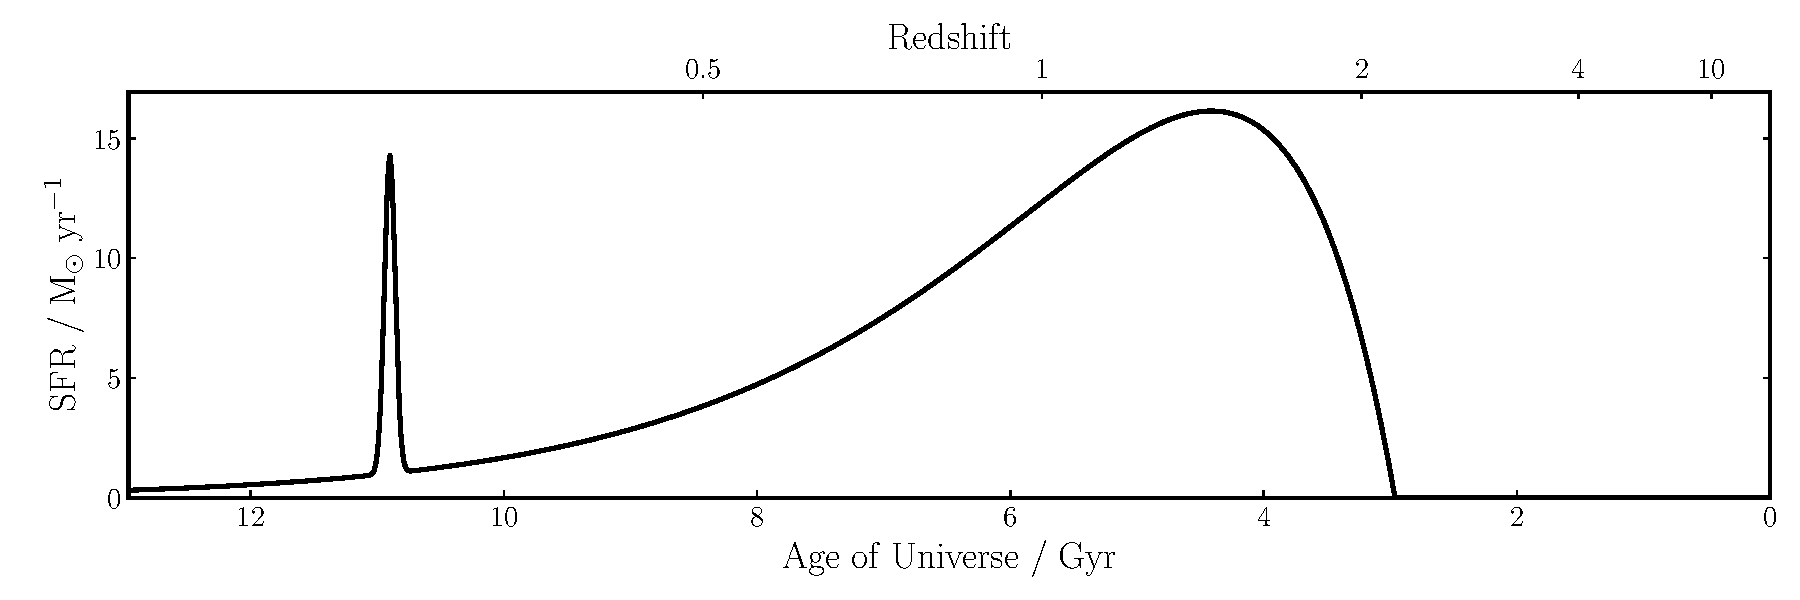
\includegraphics[width=\textwidth]{alex_model_20_sfh}
  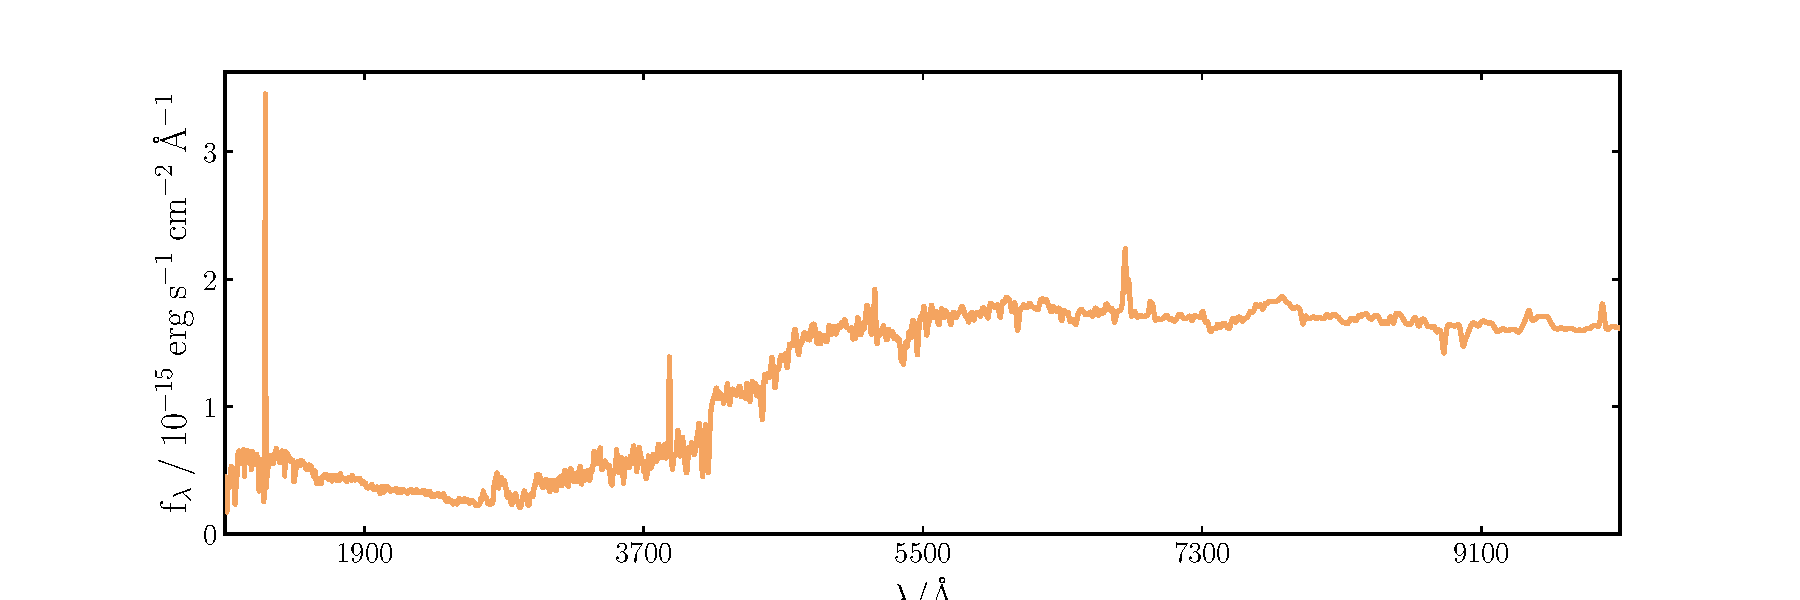
\includegraphics[width=\textwidth]{alex_model_20_spec}
  \caption{Parameterised star formation history and simulated spectrum with \textsc{Bagpipes}.}
  \label{fig:bagpipes_example_simulation}
\end{figure}

The parameter space minimally covered is:

\begin{itemize}
  \item functional form of the SFH
  \item host galaxy redshift
  \item velocity dispersion
  \item dust attenuation curve
\end{itemize}

\noindent For parameterising the SFH, \textsc{Bagpipes} allows a linear combination of one or more of several predefined functional forms. An exponentially decaying burst with form:

\begin{equation}
  \mathrm{SFR}(t) \propto
  \begin{cases}
    0 & t < T_0, \\
    e^{-\frac{t-T_0}{\tau}} & t > T_0
  \end{cases}
\end{equation}

\noindent A delayed exponentially decaying component: \textbf{TODO: DESMOS THIS!}

\begin{equation}
  \mathrm{SFR}(t) \propto
  \begin{cases}
    0 & t < T_0, \\
    (t-T_0)e^{-\frac{t-T_0}{\tau}} & t > T_0
  \end{cases}
\end{equation}

\noindent A lognormal form:

\begin{equation}
  \mathrm{SFR}(t) \propto
  \frac{1}{t\sqrt{2\pi\tau^2}}
  e^{-\frac{\left(\ln{t-t_0}\right)^2}{2\tau^2}}
\end{equation}

\noindent Defined by Gladders et al. 2013, where $t$ is the elapsed time since the big bang, $t_0$ is the logarithmic decay time, and $\tau$ sets rise and decay timescale.\cite{Gladders_2013} \textsc{Bagpipes}, however, parameterises this as $t_{max}$, the time since the big bang at the peak rate of star formation and $2\sigma$, the full width at half maximum (FWHM) of the star formation rate.\cite{Carnall_2018}

Finally, \textsc{Bagpipes} allows a more versatile double power law parameterisation:

\begin{equation}
  \mathrm{SFR}(t)\propto
  \left[
  \left(\frac{t}{\tau}\right)^{\alpha} +
  \left(\frac{t}{\tau}\right)^{-\beta}
  \right]
  ^{-1}
\end{equation}

\noindent Which usefully decouples the rising and falling slopes of the star formation, at the expense of an additional parameter in a fit which is already of high dimensionality and of increased computational resources.\cite{Carnall_2018} Each of the above parameterisations include a parameter each for the total stellar mass $m_\star$ formed by the component and the metallicity $Z$ of the stars formed. It is possible to include ``bursts'' of fixed mass such that:

\begin{equation}
  \mathrm{SFR}(t)\propto
  m_\star \delta(t-t_0)
\end{equation}

\noindent As a matter of semantics, such ``bursts'' are not necessarily synonymous with the type of ``starburst'' activity for which we are searching. The starburst component may take one of any of these forms.

Nebular Component

Velocity dispersion

Redshift

Extinction

\begin{figure}
  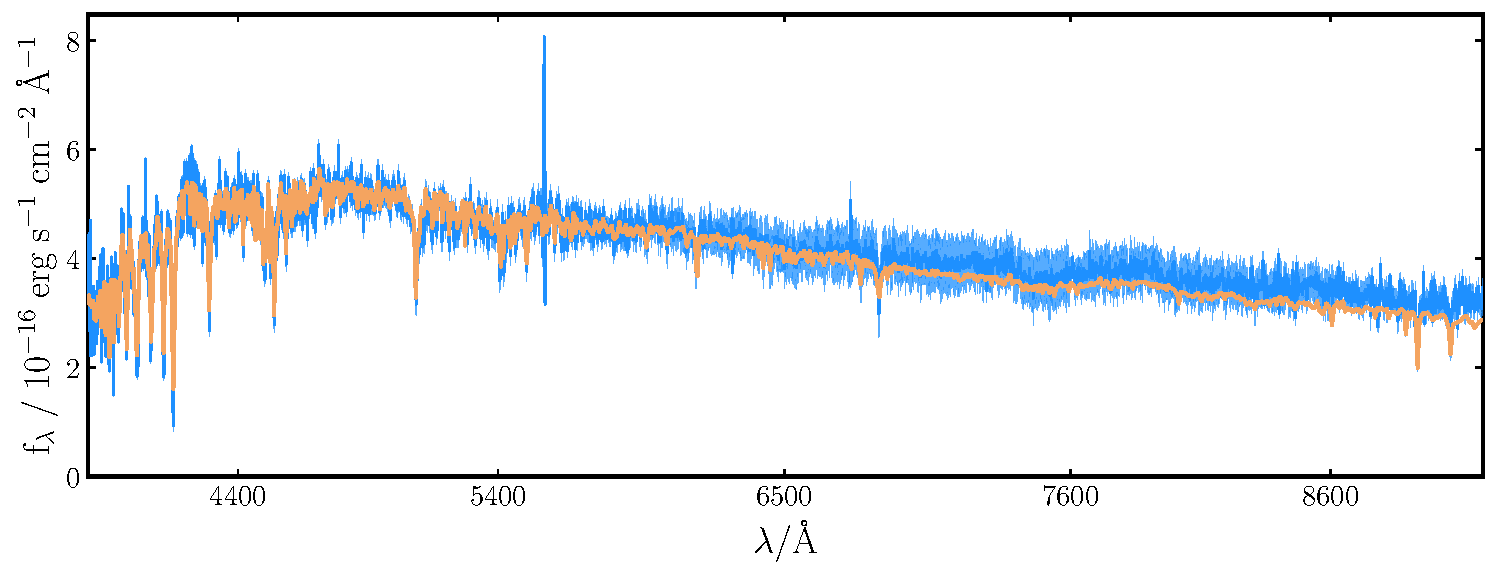
\includegraphics[width=\textwidth]{host_hyz_specwerr_fit}
  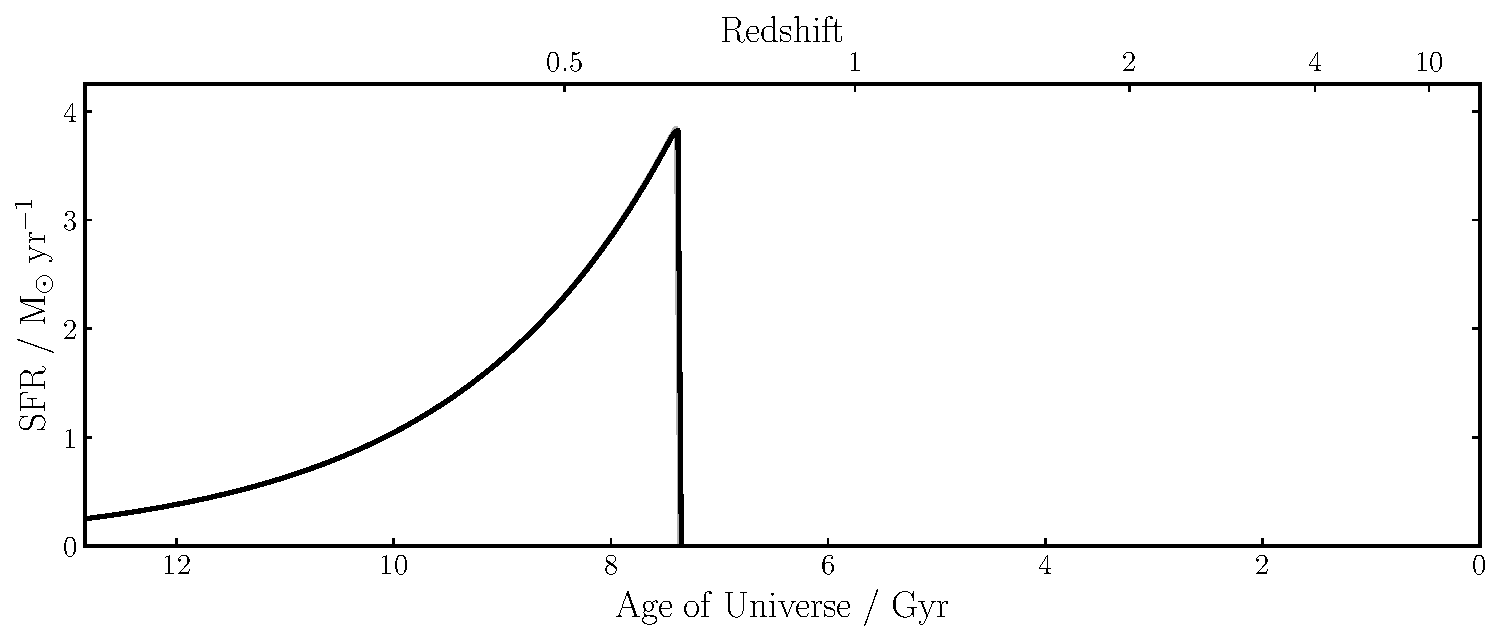
\includegraphics[width=\textwidth]{host_hyz_specwerr_sfh}
  \caption{Observed (blue) spectrum, fitted (orange) spectrum, and inferred star formation history with \textsc{Bagpipes}.}
  \label{fig:bagpipes_example_fit}
\end{figure}

\subsection{Stellar Population Fitting}\label{sec:stellar_population_fitting}

\begin{table}
  \centering
  \begin{tabular}{c c r r r}
    Spectral Type & $M/M_\odot$ & $\lambda_{peak}$     & MS Lifetime   & No. Density \\
    \hline \hline
    O5            &	40          & \SI{725}{\angstrom}  & \SI{1}{Myr}   & 1           \\
    B0            &	15          & \SI{1035}{\angstrom} & \SI{11}{Myr}  & 5           \\
    A0            &	3.5         & \SI{2898}{\angstrom} & \SI{440}{Myr} & 25          \\
    F0            &	1.7         & \SI{3864}{\angstrom} & \SI{2.7}{Gyr} & 63          \\
    G0            &	1.1         & \SI{4830}{\angstrom} & \SI{8}{Gyr}   & 100         \\
    K0            &	0.8         & \SI{5796}{\angstrom} & \SI{17}{Gyr}  & 630         \\
    M0            &	0.5         & \SI{8280}{\angstrom} & \SI{56}{Gyr}  & 800         \\
    \hline
  \end{tabular}
  \caption{Typical masses, temperatures, and main-sequence lifetimes for seven Harvard spectral subtypes. Number densities per \SI{10000}{\cubic\parsec} for each subtype's respective super-type are adapted from Glenn et al. 2001.\cite{Glenn_2001}}
  \label{tab:star_lifetimes_densities}
\end{table}

Many of the challenges in fitting spectra to SFHs are due to the limitations of stellar population fitting, whereby the total luminosity and the ratio of blue to red stars constituent in a host galaxy is used to infer the age of stellar formation components. The main sequence lifetime of a star is given by\cite{Prialnik_2010}:

\begin{equation}
  T_{MS} \propto \left(\frac{M}{M_\odot}\right)^{-2}
\end{equation}

\noindent From this we obtain the typical main-sequence lifetimes for stars of different Harvard spectral classifications, given in Table \ref{tab:star_lifetimes_densities}. From this data, the limitations of stellar population fitting are immediately apparent. Due to the inverse power law relationship between mass and main-sequence lifetime, small reductions in the initial mass (and therefore, main-sequence temperature) of stars result in dramatic increases in main-sequence lifetime. While on the main-sequence, the luminosity and colour of these long-lived stars varies little.\cite{Prialnik_2010} If, for example, the hottest stars in a stellar population are G-type stars, then stellar population fitting may reasonably find that population to be anywhere between \SI{3}{Gyr} and \SI{11}{Gyr} old. This kind of temporal resolution is comparable to the age of the universe, but star formation rates are believed to vary on much smaller timescales.\textbf{CITATION NEEDED} If star forming processes create new stars with initial masses according to some initial mass function (IMF), then star formation of sufficient total mass formed will always create some stars of each spectral type. But once the population of A-type stars, with lifetimes on the order of \SI{100}{Myr}, die out completely, it becomes increasingly difficult to pinpoint the precise age of that formation.

Indeed, calculations by Glenn et al. 2001 reproduced in Table \ref{tab:star_lifetimes_densities} show that our own Milky Way, despite being a relatively young, blue galaxy, is nevertheless mostly populated by cool red dwarves, whose lifetimes are many times that of the current age of the universe.

\section{Metal and Nebular Emission Lines}

Astrophysics of gaseous nebulae

\section{Blind Fitting with \textsc{Bagpipes}}\label{sec:blind_fitting}
Emphasize importance of computational speed. Necessity of Chi-squared selection
\subsection{R1: Wide Parameter Space with Two Components}\label{sec:r1}
For my first fitting run, I tried to first establish the functional form of the
old, bulk star formation, and then determine whether or not a more recent burst
improved the fit. I first fit each of the following functions:

\begin{tabular}{| c | c |}
  \hline
  \multicolumn{2}{| c |}{$SFR=e^{t/\tau}$} \\
  \hline
  $t$ & (3.5, 10.0) \\
  $\tau$ & (0.1, 2.0) \\
  $\log_{10}(\sfrac{M}{M_\odot})$ & (0.0, 15.0) \\
  $\sfrac{Z}{Z_\odot}$ & (0.0, 2.5) \\
  \hline
\end{tabular}

\begin{tabular}{| c | c |}
  \hline
  \multicolumn{2}{| c |}{$SFR=te^{\sfrac{-t}{\tau}}$} \\
  \hline
  $t$ & (3.5, 10.0) \\
  $\tau$ & (0.1, 2.0) \\
  $\log_{10}(\sfrac{M}{M_\odot})$ & (0.0, 15.0) \\
  $\sfrac{Z}{Z_\odot}$ & (0.0, 2.5) \\
  \hline
\end{tabular}

\begin{tabular}{| c | c |}
  \hline
  \multicolumn{2}{| c |}{$SFR=lognormal$} \\
  \hline
  $t_{max}$ & (3.5, 10.5) \\
  $2\sigma$ & (0.1, 5.0) \\
  $\log_{10}(\sfrac{M}{M_\odot})$ & (0.0, 15.0) \\
  $\sfrac{Z}{Z_\odot}$ & (0.0, 2.5) \\
  \hline
\end{tabular}

\begin{tabular}{| c | c |}
  \hline
  \multicolumn{2}{| c |}{Global Priors} \\
  \hline
  Dust Type & Calzetti \\
  $A_V$ & (0.0, 1.0) \\
  $z$ & (0.0, 0.1) \\
  $T_{bc}$ & (0.005, 0.015) \\
  $\sigma_{v}$ & (150.0, 200.0) \\
  \hline
\end{tabular}

Once the best-fit functional form of the old, bulk star formation is determined, a new fit is run with that form in linear combination with a delta function, with priors:

\begin{tabular}{| c | c |}
  \hline
  \multicolumn{2}{| c |}{$SFR=\delta_a(t)$} \\
  \hline
  $a$ & (0.1, $a_{low}$) \\
  $\log_{10}(\sfrac{M}{M_\odot})$ & (0.0, 15.0) \\
  $\sfrac{Z}{Z_\odot}$ & (0.0, 2.5) \\
  \hline
\end{tabular}
\subsection{R2 \& R3: Iterative Fitting}\label{sec:r2_and_r3}
One of the three functional forms above \textit{or} the more versatile double power law function:

\begin{equation}
  \mathrm{SFR}(t) \propto \left[ \left(\frac{t}{\tau}\right)^{\alpha} + \left(\frac{t}{\tau}\right)^{-\beta} \right]^{-1}
\end{equation}

With priors:

\begin{tabular}{| c | c |}
  \hline
  \multicolumn{2}{| c |}{$\mathrm{SFR}(t)\propto\left[\left(\sfrac{t}{\tau}\right)^{\alpha}+\left(\sfrac{t}{\tau}\right)^{-\beta} \right]^{-1}$} \\
  \hline
  $\tau$ & (0.0, 15.0) \\
  $\alpha$ & (0.0, 10.0) \\
  $\beta$ & (0.0, 10.0) \\
  $\log_{10}(\sfrac{M}{M_\odot})$ & (0.0, 15.0) \\
  $\sfrac{Z}{Z_\odot}$ & (0.0, 2.5) \\
  \hline
\end{tabular}

And with an exponentially decaying burst, the age of which is allowed to vary over a much larger parameter space:

\begin{tabular}{| c | c |}
  \hline
  \multicolumn{2}{| c |}{$SFR=e^{t/\tau}$} \\
  \hline
  $t$ & (0.0, 10.0) \\
  $\tau$ & (0.1, 2.0) \\
  $\log_{10}(\sfrac{M}{M_\odot})$ & (0.0, 15.0) \\
  $\sfrac{Z}{Z_\odot}$ & (0.0, 2.5) \\
  \hline
\end{tabular}
\subsection{Selecting Physically Reasonable Priors}\label{sec:prior_selection}

Velocity dispersion of constituent stars is allowed to vary between

The ionization parameter for nebular emission is allowed to vary between logU=-4 and logU=-2, a very low and very high rate of (molecular?) ionization.

The lifetime of the stellar birth clouds was chosen to be a normal distribution about ${t_{BC}=17Myr}$ with ${\sigma=4Myr}$, consistent with typical cloud lifetimes in the Milky Way, as determined by Murray 2011\cite{Murray_2011}.
\subsection{R4: Fixed Old Component, Free Burst Component}\label{sec:r4}
Quenching at Cosmic Noon
\begin{tabular}{| c | c |}
  \hline
  \multicolumn{2}{| c |}{$SFR=e^{t/\tau}$} \\
  \hline
  $t$ & (7.5, 12.5) \\
  $\tau$ & (0.5, 2.0) \\
  $\log_{10}(\sfrac{M}{M_\odot})$ & (5.0, 12.5) \\
  $\sfrac{Z}{Z_\odot}$ & (0.0, 2.5) \\
  \hline
\end{tabular}

\begin{tabular}{| c | c |}
  \hline
  \multicolumn{2}{| c |}{$SFR=te^{\sfrac{-t}{\tau}}$} \\
  \hline
  $t$ & (7.5, 12.5) \\
  $\tau$ & (0.1, 2.0) \\
  $\log_{10}(\sfrac{M}{M_\odot})$ & (5.0, 12.5) \\
  $\sfrac{Z}{Z_\odot}$ & (0.0, 2.5) \\
  \hline
\end{tabular}

\begin{tabular}{| c | c |}
  \hline
  \multicolumn{2}{| c |}{$SFR=lognormal$} \\
  \hline
  $t_{max}$ & (1.0, 6.0) \\
  $2\sigma$ & (0.1, 3.0) \\
  $\log_{10}(\sfrac{M}{M_\odot})$ & (5.0, 12.5) \\
  $\sfrac{Z}{Z_\odot}$ & (0.0, 2.5) \\
  \hline
\end{tabular}

\begin{tabular}{| c | c |}
  \hline
  \multicolumn{2}{| c |}{$\mathrm{SFR}(t)\propto\left[\left(\sfrac{t}{\tau}\right)^{\alpha}+\left(\sfrac{t}{\tau}\right)^{-\beta} \right]^{-1}$} \\
  \hline
  $\tau$ & (0.0, 4.5) \\
  $\alpha$ & (5.0, 10.0) \\
  $\beta$ & (5.0, 10.0) \\
  $\log_{10}(\sfrac{M}{M_\odot})$ & (5.0, 12.5) \\
  $\sfrac{Z}{Z_\odot}$ & (0.0, 2.5) \\
  \hline
\end{tabular}

And an exponentially declining burst with priors:

\begin{tabular}{| c | c |}
  \hline
  \multicolumn{2}{| c |}{$SFR=e^{t/\tau}$} \\
  \hline
  $t$ & (0.0, 3.5) \\ %Gyr, lifetime of F type stars
  $\tau$ & (0.1, 2.0) \\
  $\log_{10}(\sfrac{M}{M_\odot})$ & (0.0, 12.5) \\
  $\sfrac{Z}{Z_\odot}$ & (0.0, 2.5) \\
  \hline
\end{tabular}

\begin{tabular}{| c | c |}
  \hline
  \multicolumn{2}{| c |}{Global Priors} \\
  \hline
  Dust Type & Calzetti \\
  $z$ & ($z_{obs}-0.001$, $z_{obs}+0.001$) \\ % z varies tight_layout around z_obs.
  $\sigma_{v}$ & (50.0, 450.0) \\ % Constrained by Faber-Jackson. TODO: Lookup Minkowski 1962!
  $T_{bc}$ & (0.013, 0.021) \\  % Constraints from Murray 2011.
  $A_V$ & (0.0, 2.0) \\
  $\log{U}$ & (-4.0, -2.0) \\
  \hline
\end{tabular}
\section{Application to XSHOOTER Data}\label{sec:tde_fitting}
\section{Results \& Discussion}\label{sec:results_and_discussion}
\subsection{ASASSN-14li, $z=0.0206$}\label{sec:ASASSN-14li}

A very important discovery was made with ASASSN-14li.Initially identified in the optical, this is one of the few TDEs toshow evidence of both thermal and non-thermal components.ASASSN-14li was discovered by the All-Sky AutomatedSurvey for Supernovae(ASAS-SN; Shappee et al.2014)on2014 November 22 at the center of the nearby(z=0.0206,D=90.3 Mpc)post-starburst galaxy PGC 043234(Holoien et al.2016). PGC 043234 appears to be the remnant of a recentmerger that likely hosted a low-luminosity Type II AGN priorto the TDE(Prieto et al.2016). Holoien et al.(2016)present theoptical, UV, and X-ray properties of the event, followed byadditional X-ray(Miller et al.2015; Brown et al.2016),UV(Cenko et al.2016), radio(Alexander et al.2016; van Velzenet al.2016, and this work), and mid-IR(Jiang et al.2016)studies.\cite{Canizales_2016}

\subsection{ASASSN-15oi, $z=0.0484$}\label{sec:ASASSN-15oi}

Although the redshift was originally reported as $z=0.02$, later spectra showed that the redshift of the host galaxy is $z=0.0484$, which was used in this fit.\cite{Arcavi_2015, Holoien_2016b}
\subsection{AT2018fyk, $z=0.06$}\label{sec:AT2018fyk}
\subsection{AT2019ahk, $z=0.026211$}\label{sec:AT2019ahk}
\subsection{AT2019azh, $z=0.022$}\label{sec:AT2019azh}
\subsection{AT2019dsg, $z=0.0512$}\label{sec:AT2019dsg}
\subsection{AT2019qiz, $z=0.01513$}\label{sec:AT2019qiz}
\subsection{iPTF16fnl, $z=0.018$}\label{sec:iPTF16fnl}
Important to note that Blagorodnova et al. 2017 estimates this redshift to be $z=0.016328$, although this fit was run with $z=0.018$.\cite{Blagorodnova_2017}
\section{Conclusion}\label{sec:conclusion}
\begin{itemize}
  \item Summary
  \item Future Applications
\end{itemize}
\section{Acknowledgements}\label{sec:acknowledgements}

Special thanks to Andy Lawrence, professor at the Royal Observatory Edinburgh, for his support and advice throughout this project. Thanks also to Philip Short, a PhD candidate at the University of Edinburgh, for his preparation of the XSHOOTER data and for participating in my blind fitting trials. Thanks to Patrick Smith, for endowing me with a love of empiricism in my formative school years. And finally, thanks to my father, who even before I could stand, took me for walks under the stars.

\printbibliography

% \begin{figure}[h!]
% \centering
%   \includegraphics[width=0.9\textwidth]{../pipes/plots/priors/phil_model_01_sfh.pdf}
%   \includegraphics[width=0.9\textwidth]{../pipes/plots/lognormal_noburst/phil_model_01_sfh.pdf}
%   \includegraphics[width=0.9\textwidth]{../pipes/plots/wide_lognormal_burst/phil_model_01_sfh.pdf}
%   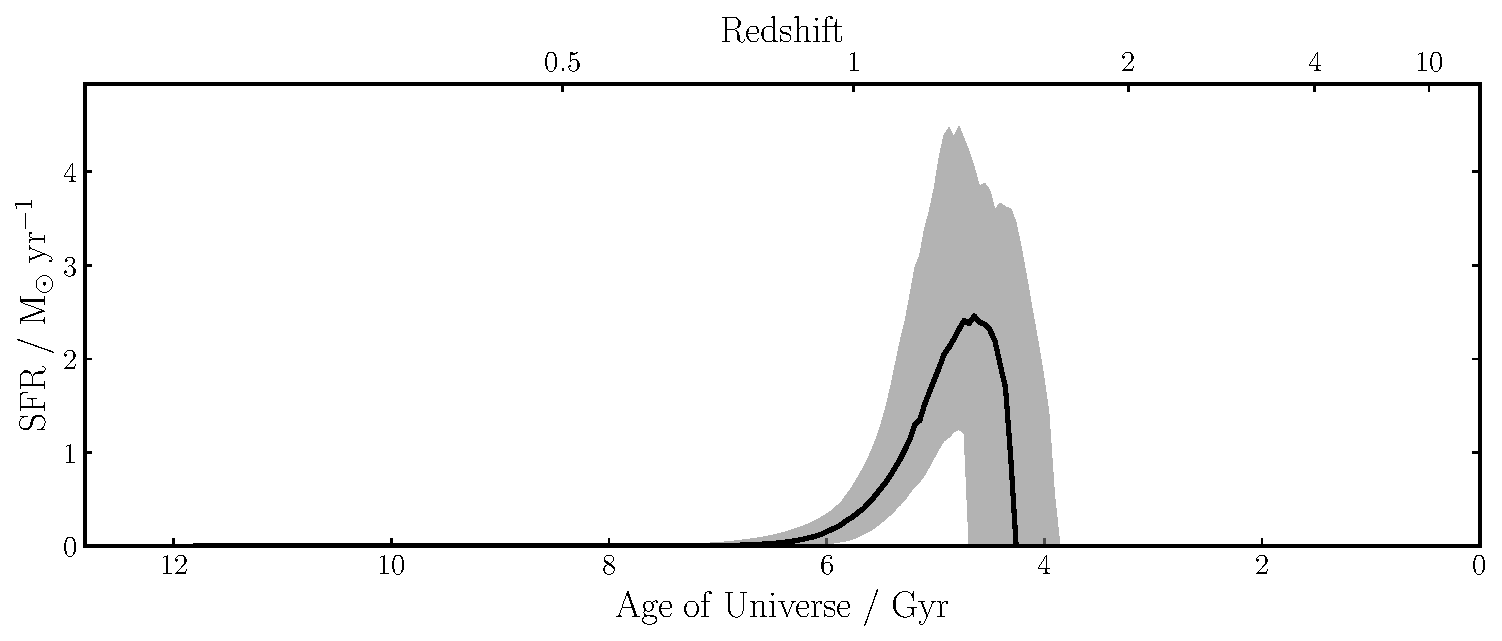
\includegraphics[width=0.9\textwidth]{../pipes/plots/lognormal_burst_final/phil_model_1_sfh.pdf}
%   \caption{A priori and posterior SFH.}
%   \label{}
% \end{figure}
%
% \newpage
% \begin{figure}[h!]
%   \centering
%   \includegraphics[width=0.9\textwidth]{../pipes/plots/priors/phil_model_02_sfh.pdf}
%   \includegraphics[width=0.9\textwidth]{../pipes/plots/exponential_burst/phil_model_02_sfh.pdf}
%   \includegraphics[width=0.9\textwidth]{../pipes/plots/wide_dblplaw_burst/phil_model_02_sfh.pdf}
%   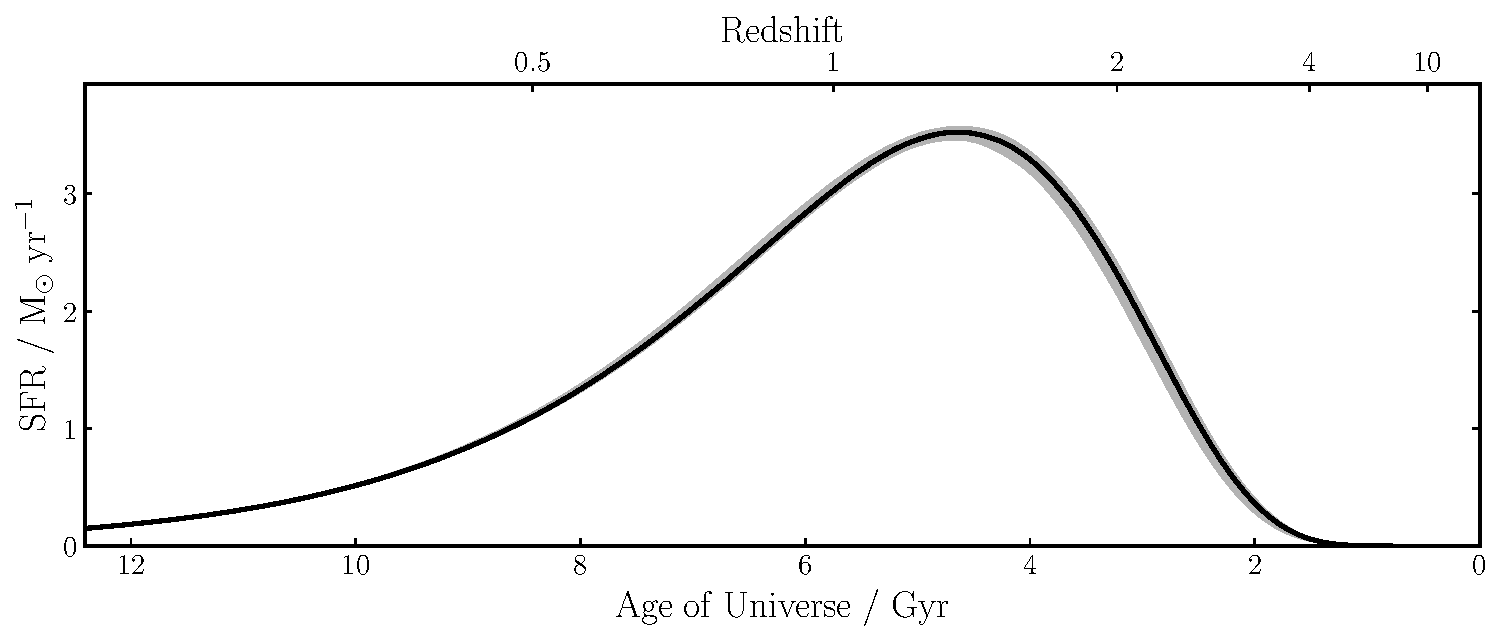
\includegraphics[width=0.9\textwidth]{../pipes/plots/exponential_burst_final/phil_model_2_sfh.pdf}
%   \caption{A priori and posterior SFH.}
%   \label{}
% \end{figure}
%
% \newpage
% \begin{figure}[h!]
%   \centering
%   \includegraphics[width=0.9\textwidth]{../pipes/plots/priors/phil_model_03_sfh.pdf}
%   \includegraphics[width=0.9\textwidth]{../pipes/plots/delayed_burst/phil_model_03_sfh.pdf}
%   \includegraphics[width=0.9\textwidth]{../pipes/plots/wide_delayed_burst/phil_model_03_sfh.pdf}
%   \caption{A priori and posterior SFH.}
%   \label{}
% \end{figure}
%
% \newpage
% \begin{figure}[h!]
%   \centering
%   \includegraphics[width=0.9\textwidth]{../pipes/plots/priors/phil_model_04_sfh.pdf}
%   \includegraphics[width=0.9\textwidth]{../pipes/plots/lognormal_burst/phil_model_04_sfh.pdf}
%   \includegraphics[width=0.9\textwidth]{../pipes/plots/wide_lognormal_burst/phil_model_04_sfh.pdf}
%   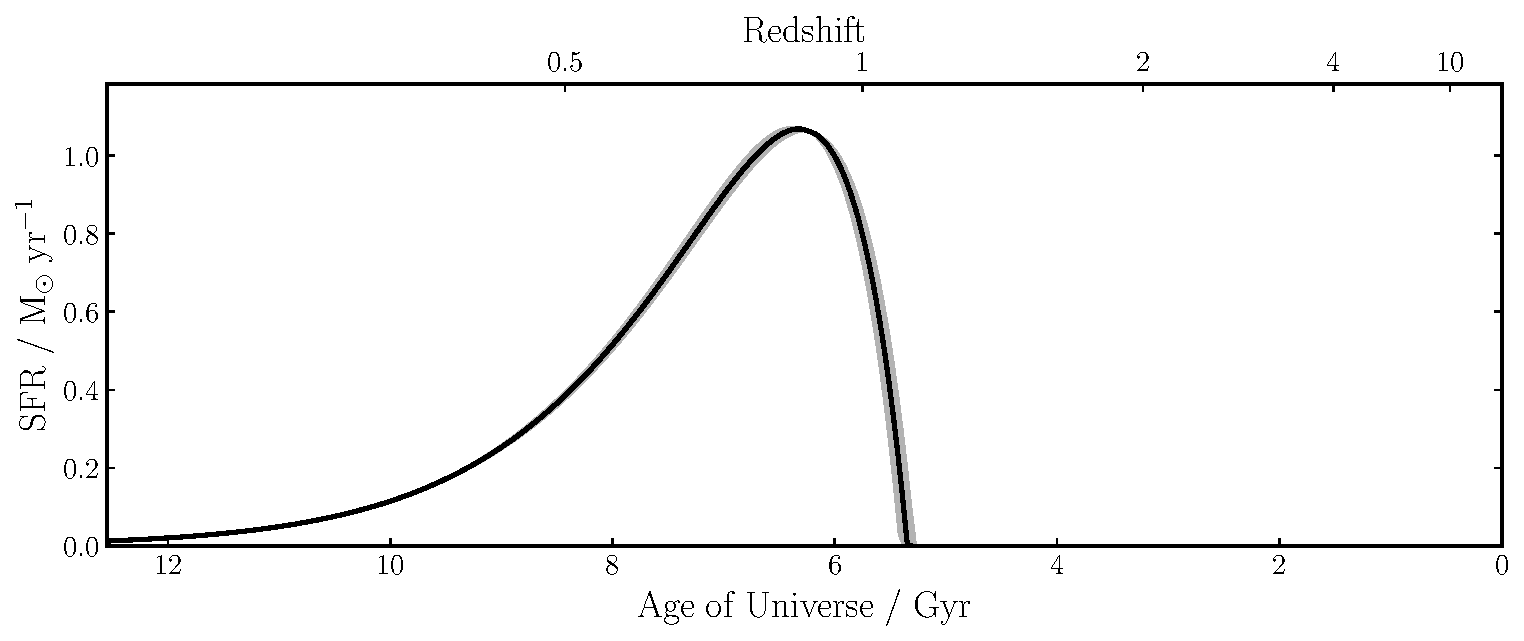
\includegraphics[width=0.9\textwidth]{../pipes/plots/exponential_burst_final/phil_model_4_sfh.pdf}
%   \caption{A priori and posterior SFH.}
%   \label{}
% \end{figure}
%
% \newpage
% \begin{figure}[h!]
%   \centering
%   \includegraphics[width=0.9\textwidth]{../pipes/plots/priors/phil_model_05_sfh.pdf}
%   \includegraphics[width=0.9\textwidth]{../pipes/plots/exponential_noburst/phil_model_05_sfh.pdf}
%   \includegraphics[width=0.9\textwidth]{../pipes/plots/exponential_noburst/phil_model_05_sfh.pdf}
%   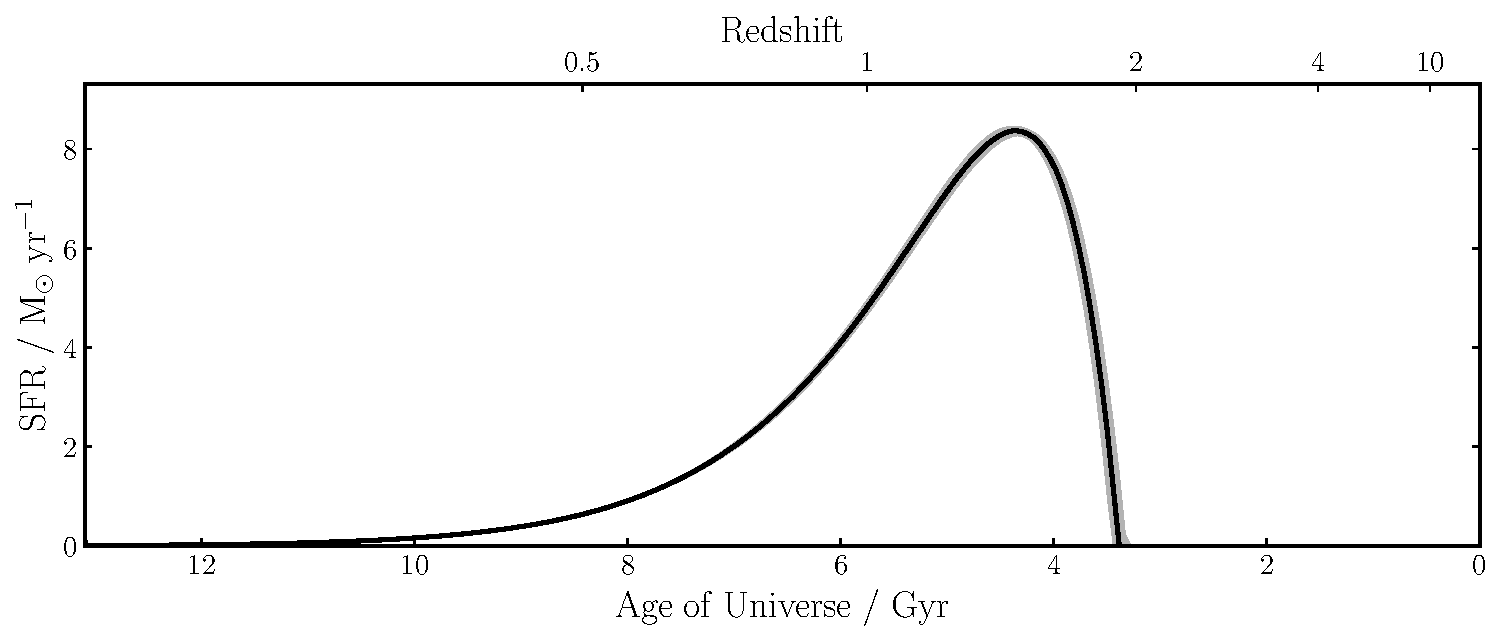
\includegraphics[width=0.9\textwidth]{../pipes/plots/delayed_burst_final/phil_model_5_sfh.pdf}
%   \caption{A priori and posterior SFH.}
%   \label{}
% \end{figure}
%
% \newpage
% \begin{figure}[h!]
%   \centering
%   \includegraphics[width=0.9\textwidth]{../pipes/plots/priors/phil_model_06_sfh.pdf}
%   \includegraphics[width=0.9\textwidth]{../pipes/plots/exponential_noburst/phil_model_06_sfh.pdf}
%   \includegraphics[width=0.9\textwidth]{../pipes/plots/wide_delayed_burst/phil_model_06_sfh.pdf}
%   \caption{A priori and posterior SFH.}
%   \label{}
% \end{figure}
%
% \newpage
% \begin{figure}[h!]
%   \centering
%   \includegraphics[width=0.9\textwidth]{../pipes/plots/priors/phil_model_07_sfh.pdf}
%   \includegraphics[width=0.9\textwidth]{../pipes/plots/exponential_burst/phil_model_07_sfh.pdf}
%   \includegraphics[width=0.9\textwidth]{../pipes/plots/wide_exponential_burst/phil_model_07_sfh.pdf}
%   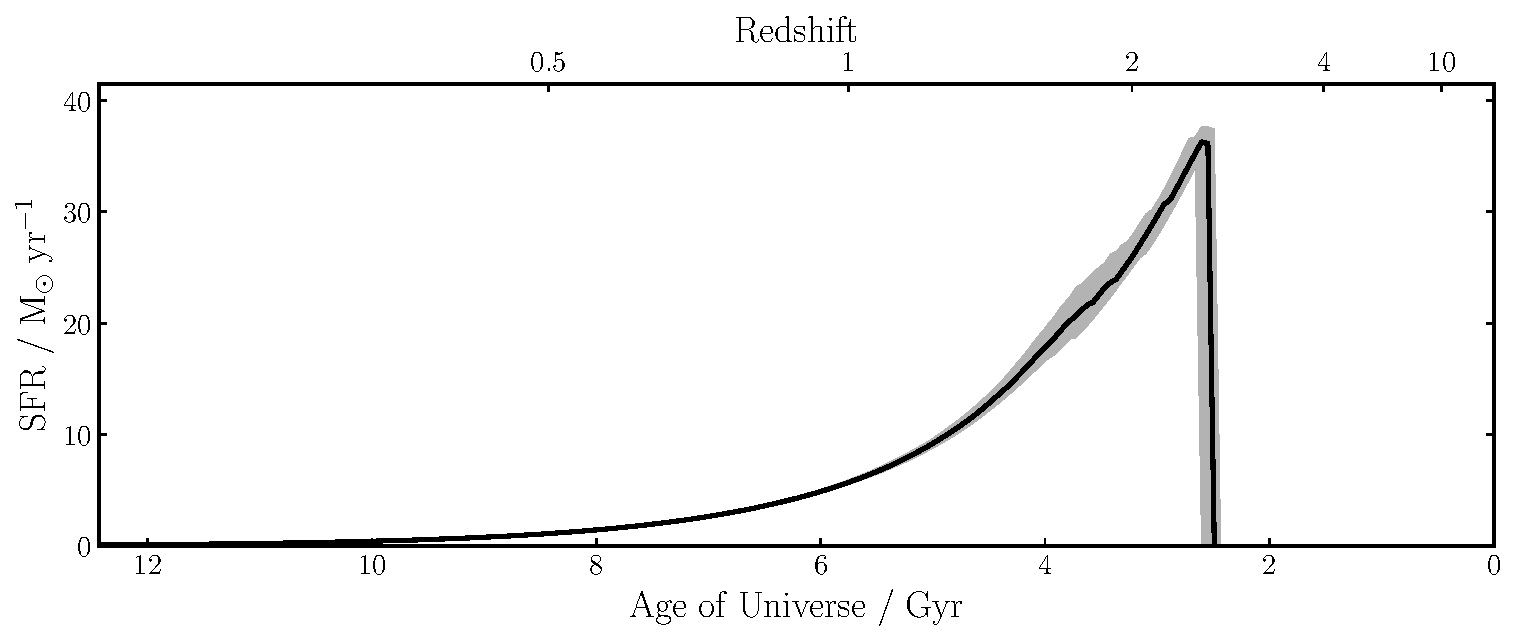
\includegraphics[width=0.9\textwidth]{../pipes/plots/delayed_burst_final/phil_model_7_sfh.pdf}
%   \caption{A priori and posterior SFH.}
%   \label{}
% \end{figure}
%
% \newpage
% \begin{figure}[h!]
%   \centering
%   \includegraphics[width=0.9\textwidth]{../pipes/plots/priors/phil_model_08_sfh.pdf}
%   \includegraphics[width=0.9\textwidth]{../pipes/plots/lognormal_burst/phil_model_08_sfh.pdf}
%   \includegraphics[width=0.9\textwidth]{../pipes/plots/wide_dblplaw_burst/phil_model_08_sfh.pdf}
%   \caption{A priori and posterior SFH.}
%   \label{}
% \end{figure}
%
% \newpage
% \begin{figure}[h!]
%   \centering
%   \includegraphics[width=0.9\textwidth]{../pipes/plots/priors/phil_model_09_sfh.pdf}
%   \includegraphics[width=0.9\textwidth]{../pipes/plots/exponential_burst/phil_model_09_sfh.pdf}
%   \includegraphics[width=0.9\textwidth]{../pipes/plots/wide_exponential_burst/phil_model_09_sfh.pdf}
%   \caption{A priori and posterior SFH.}
%   \label{}
% \end{figure}
%
% \newpage
% \begin{figure}[h!]
%   \centering
%   \includegraphics[width=0.9\textwidth]{../pipes/plots/priors/phil_model_10_sfh.pdf}
%   \includegraphics[width=0.9\textwidth]{../pipes/plots/exponential_burst/phil_model_10_sfh.pdf}
%   \includegraphics[width=0.9\textwidth]{../pipes/plots/wide_dblplaw_burst/phil_model_10_sfh.pdf}
%   \caption{A priori and posterior SFH.}
%   \label{}
% \end{figure}

\end{document}
